% Formatvorlage f�r studentische Arbeiten der Arbeitsgruppe Software Systems
% Engineering am Institut f�r Informatik der Universit�t Hildesheim
%   erstellt von Christopher Voges, 28.04.2016
%   �berarbeitet von Sascha El-Sharkawy, 06.08.2019
%   https://sse.uni-hildesheim.de/studium-lehre/richtlinien-fuer-ausarbeitungen/vorlagen/

% Dokumentenkopf 
\documentclass[
    11pt, % Schriftgr��e
    DIV=10,
    ngerman, % f�r Umlaute, Silbentrennung etc.
    a4paper, % Papierformat
    twoside, % weiseitiges Dokument
    titlepage, % es wird eine Titelseite verwendet
    parskip=half, % Abstand zwischen Abs�tzen (halbe Zeile)
    headings=normal, % Gr��e der �berschriften verkleinern
    listof=totoc, % Verzeichnisse im Inhaltsverzeichnis auff�hren
    bibliography=totoc, % Literaturverzeichnis im Inhaltsverzeichnis auff�hren
    index=totoc, % Index im Inhaltsverzeichnis auff�hren
    captions=tableheading, % Beschriftung von Tabellen unterhalb ausgeben
		numbers=noenddot,
    final, % Status des Dokuments (final/draft)
]{scrreprt}

% Einbinden der Packages
% Entfernt Probleme durch Verwendung von Koma-Script Klassen (scrreport)
\usepackage{scrhack}
% Erlaubt Konfiguration von Header & Footer
\usepackage[automark,headsepline,footsepline,plainheadsepline,plainfootsepline]{scrlayer-scrpage}

% Anpassung an Sprache (deutsch)
% \usepackage[ngerman]{babel}

% Umlaute
\usepackage[latin1]{inputenc}
\usepackage[T1]{fontenc}
\usepackage{textcomp} % Euro-Zeichen etc.

% Schrift
\usepackage{lmodern}
\usepackage{relsize}

% Einbinden von JPG-Grafiken erm�glichen
\usepackage[dvips,final]{graphicx}

% Erm�glichen mathematischer Symbole
\usepackage{amsmath,amsfonts}

% F�r die Definition der Zeilenabst�nde, Seitenr�nder etc.
\usepackage{setspace}
\usepackage{geometry}

% URL-Unterst�tzung
\usepackage{url}

% Abk�rzungsverzeichnis 
% Alles weitere hierzu in: "Inhalt\Abkuerzungen.tex".
\usepackage[intoc]{nomencl}
\let\abbrev\nomenclature
\renewcommand{\nomname}{Abk�rzungsverzeichnis}
\setlength{\nomlabelwidth}{.15\textwidth}

% PDF-Optionen -----------------------------------------------------------------
\usepackage[
    bookmarks, % Es werden Bookmarks verwendet
    bookmarksopen=true, % Farbe von Bookmarks
    colorlinks=true, % Farbe von Verkn�pfungen
    linkcolor=black, % einfache interne Verkn�pfungen
    anchorcolor=black, % Ankertext
    citecolor=black, % Verweise auf Literaturverzeichniseintr�ge im Text
    filecolor=black, % Verkn�pfungen, die lokale Dateien �ffnen
    menucolor=black, % Acrobat-Men�punkte
    urlcolor=black, % Farbe der URLs
    plainpages=false, % zur korrekten Erstellung der Bookmarks
    pdfpagelabels, % zur korrekten Erstellung der Bookmarks
    hypertexnames=false, % zur korrekten Erstellung der Bookmarks
    linktocpage, % Seitenzahlen anstatt Text im Inhaltsverzeichnis verlinken
    pdfusetitle % Erm�glicht das Setzen der Meta-Daten des erzeugten PDFs
]{hyperref}
% \renewcommand{\theHsection}{\thepart.section.\thesection}
% \hypersetup{
%     %pdftitle={\titel \untertitel},
%     pdfauthor={\autor},
%     pdfcreator={\autor}
%     %pdfsubject={\titel \untertitel},
%    % pdfkeywords={\titel \untertitel}
% }

% Wird f�r Teile der Formatierung des Deckblatts und die Verwendung von
% Aufz�hlungen ben�tigt
\usepackage{listings}
\usepackage{xcolor} 


% fortlaufendes Durchnummerieren der Fu�noten
\usepackage{chngcntr}

% bei der Definition eigener Befehle ben�tigt
\usepackage{ifthen}

% sorgt daf�r, dass Leerzeichen hinter parameterlosen Makros nicht als Makroendezeichen interpretiert werden
\usepackage{xspace}

% F�r das Erstellen eines Glossars
\usepackage[toc, automake, nonumberlist]{glossaries}

\usepackage[figure,table,lstlisting]{totalcount}

% Einbinden der Meta-Informationen
% Meta-Informationen 
% Falls Umlaute oder ein *�* vorkommen:
\usepackage[latin1]{inputenc}

% Hier k�nnen Sie Informationen zur Arbeit, sich selbst und Ihren Betreuern
% hinterlegen.
\newcommand{\titel}{Self-Adaptive Architecture in Stream Processing} % Name der Arbeit
\newcommand{\untertitel}{Untertitel} % Optional mit Untertitil
% Art der Arbeit ggf. zus�tzlich der Titel der Veranstaltung
\newcommand{\art}{Seminararbeit} 
\newcommand{\studiengang}{Angewandte Informatik (BSc)} % Ihr Studiengang
\newcommand{\autor}{Leon Meister} % Ihr Name
\newcommand{\email}{meister@uni-hildesheim.de}% Ihre aktuelle und g�ltige E-Mail-Adresse
\newcommand{\matnr}{285631} % Ihre Matrikelnummer

% Die Angaben zu uns:
\newcommand{\institut}{Institut f\"ur Informatik}
\newcommand{\arbeitsgruppe}{Arbeitsgruppe Software Systems Engineering}
\newcommand{\erstgutachter}{MSc Cui Qin, SSE}% Ihr(e) ErstgutachterIn
% \newcommand{\zweitgutachter}{<Zweitpruefer>}% Ihr(e) ZweitgutachterIn
\newcommand{\universitaet}{Universit\"at Hildesheim\ \textbullet \ Universit\"atsplatz 1 \ \textbullet \ D-31134 Hildesheim}
\newcommand{\adresse}{\arbeitsgruppe \ \textbullet \ \institut \\ \universitaet}

\newcommand{\version}{Version 1.0}% Die Version der Arbeit

% Wird 'projektarbeit' auf 'true' gesetzt, wird keine Eigenst�ndigkeitserkl�rung
% erzeugt.
\newboolean{projektarbeit}
\setboolean{projektarbeit}{false}

% Wird 'final' auf 'true' gesetzt, werden folgende �nderungen vorgenommen:
% -Entfernen von Datum in der Kopf- und Versionsnummer in der Fu�zeile
% -Entfernen von Datum und Versionsnummer vom Deckblatt
% -Es werden Leerseiten f�r den doppelseitigen Druck eingef�gt
\newboolean{final}
\setboolean{final}{false}





% Erstellung der Verzeichnisse und Glossars aktivieren
\makeindex
\makenomenclature
\makeglossaries 
\glstoctrue 


% Kopf- und Fu�zeilen, Seitenr�nder etc. anpassen
% Zeilenabstand: einfach 
\newcommand{\zeilenabstandHauptteil}{1.0}
\newcommand{\zeilenabstandAnhang}{1.0}

% Seitenr�nder
\setlength{\topskip}{\ht\strutbox} % behebt Warnung von geometry
% Initiales Papierformat, wird nach dem Deckblatt teilwiese ge�ndert 
\geometry{paper=a4paper,left=3.5cm, right=2.5cm, top=2.5cm, bottom=2.9cm, headsep=.6cm}

%% Einstellen der Schriftgr��en der �berschriften
\setkomafont{chapter}{\LARGE\bfseries\rmfamily}
\setkomafont{section}{\Large\bfseries\rmfamily}
\setkomafont{subsection}{\large\bfseries\rmfamily}
\setkomafont{subsubsection}{\large\mdseries\rmfamily}
\setkomafont{pageheadfoot}{\normalfont}

%% Einstellen der Abst�nde vor und nach den �berschriften
\RedeclareSectionCommand[
  %runin=false,
  afterindent=false,
  beforeskip=0pt,
  afterskip=.05\baselineskip]{chapter}
\RedeclareSectionCommand[
  %runin=false,
  afterindent=false,
  beforeskip=0pt,
  afterskip=.05\baselineskip]{section}
\RedeclareSectionCommand[
  %runin=false,
  afterindent=false,
  beforeskip=0pt,
  afterskip=.05\baselineskip]{subsection}
\RedeclareSectionCommand[
  %runin=false,
  afterindent=false,
  beforeskip=0pt,
  afterskip=.05\baselineskip]{subsubsection}

% Header & Footer konfigurieren
\renewcommand*{\chaptermarkformat}{} % Keine Nummerierung im Header
\clearpairofpagestyles % Voreinstellungen l�schen
% E = Even page  (Gerade Seitennummer)
% O = Odd page   (Ungerade Seitennummer)
% L = Left side	 (Linker Teil der Seite)
% C = Centered   (Mittlerer Teil der Seite)
% R = Right side (Rechter Teil der Seite)
% Auf ungeraden Seiten: Kapitel�berschrift, oben rechts
\rohead[\leftmark]{\leftmark}
% Auf geraden Seiten: Titel der Arbeit, oben links
\lehead[\titel]{\titel}
% Seitenzahlen in der Mitte eines Zweiseitigenausdrucks
\rofoot[\thepage]{\thepage}
\lefoot[\thepage]{\thepage}

\ifthenelse{\boolean{final}}{% Keine besondere Aktion in der finalen Fassung
  } {
		%Versionsnummer f�r Draft
		\lohead[Version vom \today~(Vor Abgabe entfernen)]{Version vom \today~(Vor Abgabe entfernen)}
		\rehead[Version vom \today~(Vor Abgabe entfernen)]{Version vom \today~(Vor Abgabe entfernen)}
		\lofoot[Version vom \version~(Vor Abgabe entfernen)]{Version vom \version~(Vor Abgabe entfernen)}
		\refoot[Version vom \version~(Vor Abgabe entfernen)]{Version vom \version~(Vor Abgabe entfernen)}
	}

% erzeugt ein wenig mehr Platz hinter einem Punkt
\frenchspacing 

% Schusterjungen und Hurenkinder vermeiden
\clubpenalty = 10000
\widowpenalty = 10000 
\displaywidowpenalty = 10000

% Quellcode-Ausgabe formatieren
\lstset{numbers=left, numberstyle=\tiny, numbersep=5pt, breaklines=true}
\lstset{emph={square}, emphstyle=\color{red}, emph={[2]root,base}, emphstyle={[2]\color{blue}}}

% Fu�noten fortlaufend durchnummerieren
\counterwithout{footnote}{chapter}

% Einstellungen f�r Listings
\definecolor{hellgelb}{rgb}{1,1,0.9}
\definecolor{colKeys}{rgb}{0,0,1}
\definecolor{colIdentifier}{rgb}{0,0,0}
\definecolor{colComments}{rgb}{1,0,0}
\definecolor{colString}{rgb}{0,0.5,0}
\lstset{
    float=hbp,
    columns=flexible,
    tabsize=2,
    frame=single,
    extendedchars=true,
    showspaces=false,
    showstringspaces=false,
    numbers=left,
    numberstyle=\tiny,
    breaklines=true,
    breakautoindent=true,
    xleftmargin=0.6cm,
    xrightmargin=0.1cm,
    captionpos=b
}

% Eigene Definitionen f�r Silbentrennung laden
% Trennvorschl�ge im Text werden mit \" angegeben
% untrennbare W�rter und Ausnahmen von der normalen Trennung k�nnen in dieser
% Datei mittels \hyphenation definiert werden


% Eigene LaTeX-Befehle laden
% Eigene Befehle, z.B.:
\newcommand{\fett}[1]{\textbf{#1}}

% Hier beginnt das eigentliche Dokument
\begin{document}
\title{\titel}
\author{\autor}

% Setzt wie tief Abschnitte numeriert und ins Inhaltsverzeichnis
% aufgenommen werden sollen, hier: bis inkl. SubSubSection (z.B. 1.1.1.1).
\setcounter{secnumdepth}{3}
\setcounter{tocdepth}{3}

% Deckblatt einbinden
% Erzeugt das Deckblatt
%   Bei zu langem Arbeitstitel m�ssen die vertikalen Abst�nde (\vspace)
%   angepasst werden, damit das Deckblatt weiterhin auf eine Seite passt.
\begin{titlepage}
\newgeometry{top=2cm,bottom=2cm,left=2cm,right=2cm}
\begin{figure}
    
\includegraphics[scale=0.22]{Bilder/SSE_logo_2000_resized.pdf}
		\hfill
		
\includegraphics[scale=0.25]{Bilder/St_Uni-Logo-9-2003-eps-converted-to.pdf}
\end{figure}
\begin{center}
    \vspace*{0cm}
    \huge{\textbf{\art~im Studiengang \studiengang}}
\end{center}
\begin{center}
    \vspace{1cm}
    \Huge{\textbf{\titel}}
    \vspace{1cm}
\end{center}
\ifthenelse{\boolean{final}}{}{
    \begin{center}
        \version ~vom \today\\
        (Vor Abgabe entfernen)
    \end{center}
}
\begin{center}
    \vspace{1cm}
    \huge{\textbf{\autor\\}}
    \vspace{1cm}
    \LARGE{\matnr\\}
    \vspace{0,5cm}
    \LARGE{\email}
\end{center}
\vspace{1cm}
\begin{center}
    \centering
    \LARGE{\textbf{Betreuer:}} \\
    \LARGE{\erstgutachter} \\
    \LARGE{\zweitgutachter} ~\\
\end{center}
\vspace{0.5cm}
\begin{flushright}
\end{flushright}
\begin{center}
    \small{\arbeitsgruppe \ \textbullet \ \institut \\ Universit\"at Hildesheim
    \textbullet \ Universit\"atsplatz 1 \textbullet \ D-31134 Hildesheim}
\end{center}
\end{titlepage}
\restoregeometry

% Setzen des Papierformats f�r den Rest des Dokuments
%\newgeometry{left=3.5cm, right=2.5cm, top=2.9cm, bottom=2.9cm}

% Bei finaler Fassung: Leere Seite als R�ckseite des Deckblatts 
\ifthenelse{\boolean{final}}{\cleardoublepage}{} 

% Selbstst�ndigkeitserkl�rung einbinden
\ifthenelse{\boolean{projektarbeit}}{}{\thispagestyle{empty}
\vspace*{.5cm}
\Large \textbf{Eigenst�ndigkeitserkl�rung} \normalsize
\begin{verbatim}
\end{verbatim}\setstretch{1.20}
% Bei abweichender Vorgabe bspw. durch Ihr Pr�fungsordnung, muss der
% nachfolgende Text durch den vorgegeben ersetzt werden!
\fett{Erkl�rung �ber das selbstst�ndige Verfassen von "\titel"}

Ich versichere hiermit, dass ich die vorstehende Arbeit selbstst�ndig verfasst
und keine anderen als die angegebenen Hilfsmittel benutzt habe. Die Stellen der obigen Arbeit, die anderen Werken dem Wortlaut oder dem Sinn nach entnommen wurden, habe ich in jedem Fall durch die Angabe der Quelle bzw. der Herkunft, auch der benutzten Sekund�rliteratur, als Entlehnung kenntlich gemacht. Dies gilt auch f�r Zeichnungen, Skizzen, bildliche Darstellungen sowie f�r Quellen aus dem Internet und anderen elektronischen Text- und Datensammlungen und dergleichen. Die eingereichte Arbeit ist nicht anderweitig als Pr�fungsleistung verwendet worden oder in deutscher oder einer anderen Sprache als Ver�ffentlichung erschienen. Mir ist bewusst, dass wahrheitswidrige Angaben als T�uschung behandelt werden.

Hildesheim, den~\today

\unitlength 5mm
\begin{picture}(5,4) \put(0,0) {\line(1,0){22}} \end{picture}\\
\autor
}

% Bei finaler Fassung: Leere Seite als R�ckseite der Erkl�rung
\ifthenelse{\boolean{projektarbeit}}{}{\ifthenelse{\boolean{final}}{\cleardoublepage}{}}

% Abstract einbinden
% Vor dem Hauptteil werden die Seiten in gro�en r�mischen Ziffern nummeriert.
\pagenumbering{roman}

% \section*{Kurzfassung}
% \label{sec:Kurzfassung}
% Eine kurze Zusammenfassung der Arbeit, die Interesse beim Leser wecken soll. 


\section*{Abstract}
\label{sec:Abstract}
Due to the ever increasing amount of generated data and the importance of data, stream processing systems are becoming more prevalent.
However, as data flows are not steady, a system often times is faced with over- or under utilization of its resources. 
Manual reconfiguration of stream processing applications, however, is hard and time-consuming.
In this thesis we explore self-adaptive stream processing systems as a means to overcome these problems. 
Our goal is to gain an overview of the topic of self-adaptive stream processing systems and to analyze two viable architectural patterns for such systems.



% Bei finaler Fassung: Leere Seite als R�ckseite des Abstracts
\ifthenelse{\boolean{final}}{\cleardoublepage}{}

% Verzeichnisse drucken
\tableofcontents% Inhaltsverzeichnis

% Wenn Abbildungs- und Tabellenverzeichnis auf die selbe Seite sollen: 
\iftotalfigures\listoffigures\fi
\begingroup 
\let\clearpage\relax
\vspace{1cm} 
\iftotaltables\listoftables\fi
\endgroup
 
% Wenn Abbildungs- und Tabellenverzeichnis je auf einer eigenen Seite beginnen
% sollen: 
% \listoffigures % Abbildungsverzeichnis
% \listoftables % Tabellenverzeichnis

% Erstellen des Liste der Listings
\renewcommand{\lstlistlistingname}{Quellcode-Verzeichnis}
\iftotallstlistings\lstlistoflistings\fi

% Abk�rzungsverzeichnis einbinden
\nomenclature{DBMS}{Data Base Management System}
\nomenclature{DSMS}{Data Stream Management System}
\nomenclature{SPS}{Stream Processing System}
\nomenclature{DPS}{Data Stream Processing}
\nomenclature{EDF}{Elastic and Distributed DSP Framework}
\nomenclature{IDC}{International Data Corporation}
\nomenclature{I/O}{Input/Output}

% F�r korrekte �berschrift in der Kopfzeile
\clearpage\markboth{\nomname}{\nomname}

% Drucken des Abk�rzungsverzeichnises
\printnomenclature
\label{cha:Abkuerzungsverzeichnis}
 
% Arabische Seitenzahlen im Hauptteil 
\ifthenelse{\boolean{final}}{\cleardoublepage}{\clearpage}
\pagenumbering{arabic}

% Die Inhaltskapitel aus "Inhalt.tex" einbinden
\begin{spacing}{\zeilenabstandHauptteil}
% Hier k�nnen die einzelnen Kapitel inkludiert werden. 
% Die Dateien m�ssen auf .tex enden. Diese Endung muss
% beim Inkludieren aber weggelassen werden.
% Info: \include und \input unterscheiden sich im wesentlichen darin, dass bei
% \include immer eine neue Seite angefangen wird.

\chapter{Introduction}
\label{cha:Introduction} % Ein Label ist optional, ermoeglicht aber die Referenzierung
\textbf{\color{red}THIS IS NOT FINAL}

NOTES:
Motivation
Goal -> Research question definieren und spezifizieren, discuss the different architectures
Struktur erläutern

% Introduction: lots of data -> cant save it all -> need a way to deal with it
% Examples of when it is applied
% How does it work, are there alternatives? yes -> batch processing (Maybe briefly explain)
The advancements in technology of the past decades has lead to enormous data creation. Technology has become ubiquitous, 
with the evolution of cell phones to smartphones, the digitilization of industrial processes, Industry 4.0
and the increasing amount of ``smart`` devices, causing creation of information to grow exponentially.
It is estimated that the \gls{datasphere} will reach the size of 175 zettabytes by 2025, as shown in figure 1.1.
% Graph estimating the growth of the global datasphere (by IDC)
\begin{figure}[ht]
\centering
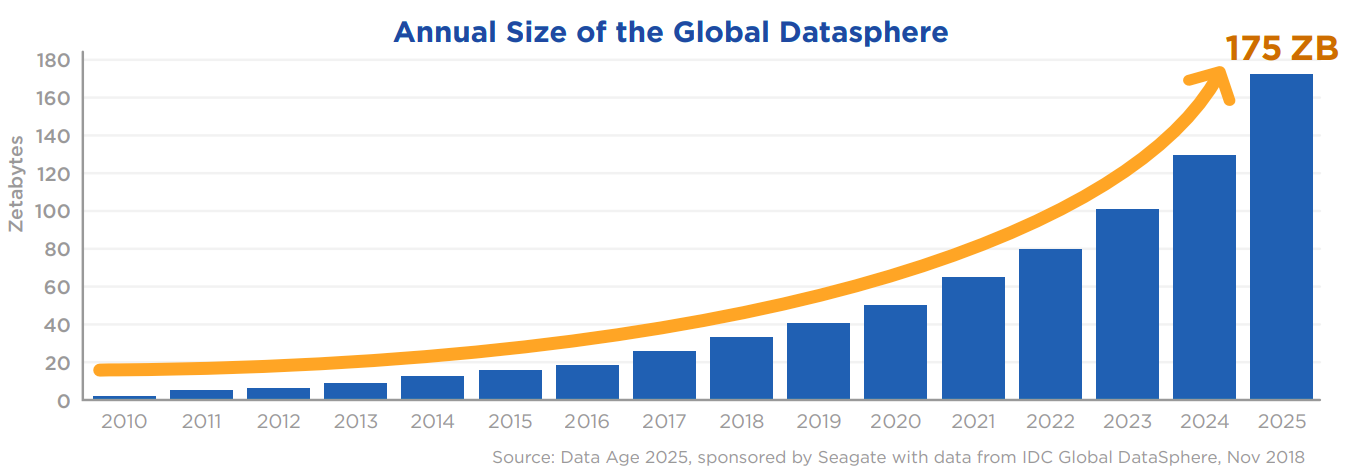
\includegraphics[width=1.0\textwidth]{Bilder/size_global_datasphere.png}
\caption{The Growth of the Global Datasphere \cite[p.6]{idc-seagate-data}}
\label{fig:growth_datasphere}
\end{figure}

% Maybe a source here?
Data has become an important factor in decision making and optimization in virtually every industry, especially in finances. \fett{TODO: Wieso?}
The financial market is dominated by data driven decisions, with emphasis on data processing in a (near) real-time fashion.
However, real-time data is becoming of importance in multiple sectors; the International Data Corporation estimates that real-time data will be 
responsible for a share of 30 percent of the total global datasphere by 2025, as shown in figure 1.2.
% Graph showing the growing share of real-time data as part of global datasphere
\begin{figure}[h]
\centering
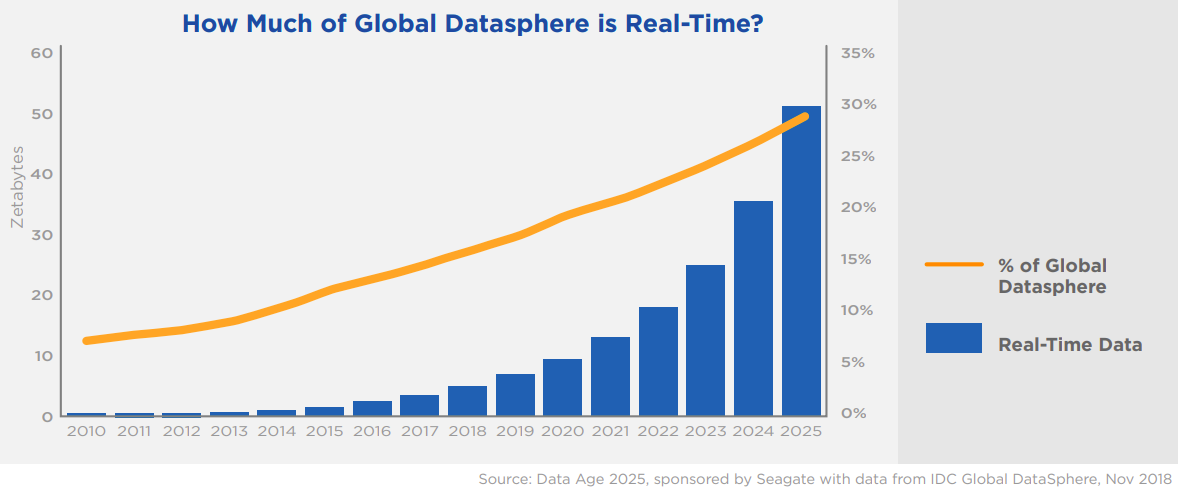
\includegraphics[width=1.0\textwidth]{Bilder/realtime_data.png}
\caption{The growth of real-time data as part of the Global Datasphere \cite[p.13]{idc-seagate-data}}
\label{fig:growth_realtime_data}
\end{figure}

A global study led by IBM in 2012 has shown that 71 percent of the firms in the financial market use information (including big data)
in order to achieve an advantage over their competitors, compared to 36 percent, which IBM has found in an earlier study conducted in 2010. \cite[p.1]{ibm-financial}

As it is no longer feasible to save all the data before then analyzing it (in batches), due to computational cost and lack of storage capacity, 
a new approach was designed in order to handle data in a (near) real-time fashion, Stream Processing Systems (SPS).

\fett{TODO: Why self adaptivity is needed? Research different kinds of adaptation (e.g. load shedding, elastric allocation of resources), look at cui's paper, add concrete examples
Structure:
Why stream processing? -> Why adaptive?}
\chapter{Fundamental Concepts}
\textbf{TODO: In this chapter we...}
This chapter lays out the fundamental concepts that are needed in order to discuss the topic.

    \section{Stream Processing}
    In this section I will split the concept of Stream Processing into three further components.
    In 2.1.1 I will then define Stream Processing Systems, explain how they work and give examplary fields of application.
    Afterwards in 2.1.2 I will then move onto the topic of Data Stream Management Systems and finally in 2.1.3 I will talk about
    some requirements that SPS should meet.
    
        \subsection{Stream Processing Systems}
        This subsection should explain what stream processing systems are, how they work, what kind of SPS are around
        \textbf{TODO: Wie sieht Data in SPS aus? discuss with DBMS approach, too}
        An SPS takes in one or multiple continuous streams of data, each element of the stream then gets processed by a number of operators and eventually, 
        the SPS puts out a stream of processed data.
    
        In order to increase efficiency, an SPS can, if (computational) resources are available, create replicas of operators to introduce parallelity. 
        Conversely, if there is little input, it may also reduce the amount of replicas in order to save or free up additional resources, as shown in figure 2.1.
        \begin{figure}[h]
        \centering
        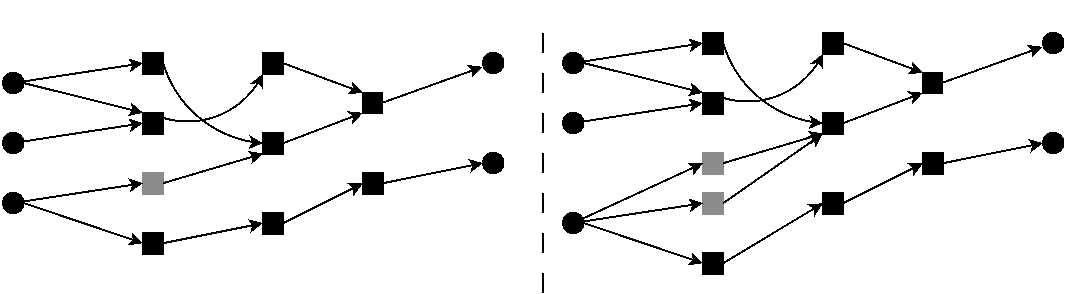
\includegraphics[width=1.0\textwidth]{Bilder/sps_parallel_normal.png}
        \caption{
                Left: An example for an SPS displayed as a directed acyclic graph. 
                Right: Same SPS with introduced parallelity in one operator, marked gray for visibility. 
                Circles are input/outputs, squares are operators, arrows are streams.
                }
        \label{fig:sps_parallel_normal}
        \end{figure}
        \subsection{Data Stream Management Systems}
        what are dsms, why dsms as opposed to dbms

        % Subsection Requirements for Stream Processing Systems
        % Should quickly go over the requirements and explain why they matter to us
        \subsection{Requirements for Stream Processing Systems}
        What are the requirements, why do they matter to us (Elaborate on this)

        Due to the nature of the fields in which SPS are used, there are important requirements that SPS should meet in order to be viable, 
        which Stonebraker et al. point out in \cite{Stonebraker:2005:RRS:1107499.1107504}, of which the ones most important to us can be summarized as the following:
        
        % Enumeration of requirements for SPS + explanations why they matter to us
        \begin{enumerate}
            \item \textbf{Keep the Data Moving:} 
                In order to minimize latency, data must not be stored, as these are costly operations.
            \item \textbf{Handle Stream Imperfections:} 
                Expecting only perfect data is utopian, so one must prepare the system with built-in mechanisms for data that might be missing or out-of-order.
            \item \textbf{Integrate Stored and Streaming Data:} 
                For an SPS to be able to perform comparisons between "predecessor" data and current data, operators must keep an efficiently manageable state.
            \item \textbf{Guarantee Data Safety and Availability:} 
                Recovering from a failure is detrimental for real-time data processing, so a system must be in place to guarantee the highest availability possible.
            \item \textbf{Process and Respond Instantaneously:} 
                Systems must be highly optimized in order to provide (near) real-time responses.
            \item \textbf{Partition and Scale Applications Automatically:} 
                Systems must be able to be split across multiple machines and threads.
                The system must also be able to automatically scale and distribute the load across the machines.

        \end{enumerate}

    \section{MAPE-K Loop}
    % Explain the MAPE-K Loop as it is a valuable basis/reference architecture for many different approaches in adaptive systems
    % Rough explanation of what it is, where it is used
    % explain different "stages" (m, a, p, e)
    % Explain -K extension
    The MAPE-K Loop was introduced by IBM \cite{Kephart:2003:VAC:642194.642200}
    and refers to a proposed solution for self-adaptive or autonomic systems.
    This model has since become the basis or reference architectural pattern for many self adaptive systems, which I will show in the third chapter.
    The acronym MAPE-K refers to the components that make up the model:
    \begin{enumerate}
        \item \textbf{M}onitor: 
            The \textit{Monitor} component gathers data about the system and its environment, aggregates and filters it.
            As soon as a symptom is encountered that needs to be analyzed, the information is forwarded to the \textit{Analyze} component.
        \item \textbf{A}nalyze: 
            The \textit{Analyze} component analyzes the previously gathered data and determines whether or not an adaptation should be performed.
            The decision is made based on performance or cost gain and should include the adaptation cost as well.
            This component's analysis is influenced by the \textit{Knowledge} base.
        \item \textbf{P}lan: 
            If the choice to adapt the system has been made, the \textit{Plan} component then decides how to reconfigure the system.
            Once the decision has been made, the information is then forwarded to the \textit{Execute} component.
        \item \textbf{E}xecute: 
            Given the \textit{Plan} component's decision, the \textit{Execute} component then executes said plan and the loop 
            returns to the initial monitoring state.
        \item \textbf{K}nowledge: 
            Represents the knowledge base, which is shared between the other components.
            This base is created by the \textit{Monitor} component and contains information in the form of metrics, policies, symptoms and logs.
    \end{enumerate}

    
    \section{Self-Adaptive Systems}
    This subchapter should explain what self-adaptive systems are and how they function.
    What kind of self-adaptive systems are around?

    % Definition of self-adaptive systems
    % Architecture often based on mape in different patterns
    % applied in xx industries
    Cheng et al define self-adaptive systems as
    \begin{quotation}
        ``[...] systems that are able to adjust their behaviour in response to their perception of the environment and the
        system itself [...]``\cite[p.1]{Cheng:2009:SES:1573856.1573858}.
    \end{quotation}

    





\chapter{Approaches for Self-Adaptive Architectures in Stream Processing}
Explain that this chapter showcases a few select strategies, which are then elaborated on further in the subchapters
Question: Even more approaches? e.g. Master-Slave pattern or Coordinated Control pattern (Both MAPE based)?
\textbf{Add and explain a few more MAPE Based architectures}

    \section{Dhalion}
    Quick Introduction to Dhalion, this chapter will deal with the Dhalion paper.

        \subsection{An Outline of Heron}
        Small outline of Heron, as Dhalion is built on top of Twitter's Heron.

        \subsection{Dhalion's Architecture}
        Explanation of Dhalion's Architecture \textbf{KERNPUNKT DER SECTION DHALION}

        \subsection{Discussion of Dhalion}
        Discuss the approach and compare it to the reference architecture (Mape?)
        \textbf{TODO: Maybe discuss how they evaluate, look at metrics relevant to architecture}

    \section{Hierarchical Control Architectures}
    Quick Introduction to hierarchical control architectures, this chapter deals with the Cardellini
    paper (An example for such an architecture)

        \subsection{Elastic and Distributed DSP Framework}
        Explanation of the EDF Architecture, their approaches

        \subsection{Possible Solutions for Controlling the Adaptation of Data Stream Processing Operators}

        \subsection{Discussion of EDF}

    \section{Title??}
    \textbf{TODO: Discuss among all of them, critical thinking..}

    \textbf{TODO: If enough material compare the architecture relevant metrics of the approaches}
\chapter{Summary And Conclusion}
In this chapter we will summarize the findings of the paper in \ref{sec:summary}, as well as draw a conclusion in \ref{sec:conclusion}.
\label{cha:summary}
\section{Summary}
\label{sec:summary}
In this section we will summarize the findings per chapter.

\quad In chapter \ref{cha:introduction}..
% why stream processing is needed
% why self-adaptivity is needed

\quad In chapter \ref{cha:fundamentals}..
% explained stream processing
% dsmsm
% what streams are
% what self-adaptivity is
% possible use cases
% mape loop

\quad In chapter \ref{cha:approaches}..
% explained two different approaches
% dhalion
% hierarchical control EDF...


\section{Conclusion}
\label{sec:conclusion}
Conclude the paper


\end{spacing}

% Die Inhalte des Anhangs werden analog zu den Kapiteln eingebunden.
% Wenn kein Anhang vorhanden ist, m�ssen die n�chten 7 Zeilen auskommentiert
% werden (bis '\end{spaching}').
\begin{spacing}{\zeilenabstandAnhang}
\appendix
    \chapter{Anhang}
    \label{sec:Anhang}
    % Hier k�nnen die einzelnen Anh�nge inkludiert werden. 
% Die Dateien m�ssen auf .tex enden. Diese Endung muss
% beim inkludieren aber weggelassen werden.
% Info: \include und \input unterscheiden sich im wesentlichen darin, dass bei
% \include immer eine neue Seite angefangen wird.
\section{Beispiele}
Zitat ohne Seitenangabe: \cite{BoeckleKnauberPohl+04}

Zitat mit Seitenangabe: \cite[S.1]{BoeckleKnauberPohl+04}

Referenz eines Glossareintrags: \gls{computer}

Eine normale Liste:
\begin{itemize}
\item Ein Punkt
\item Ein anderer Punkt
\end{itemize}

Eine nummerierte Liste:
\begin{enumerate}
\item Erstens
\item Zweitens
\item \ldots
\end{enumerate}

Eine Tabelle:
\begin{table}[h]
    \centering
    \captionabove{Eine Tabelle} 
    \label{tab:bspTabelle}
    \begin{tabular}{|c|c|c|} \hline
        Spalte 1 & Spalte 2 & Spalte 3 \\ \hline
        1 & 2 & 3 \\ \hline
    \end{tabular}
\end{table}

\textbf{Fetter Text}

\textit{Kursiver Text}

Eine Referenz: Siehe Tabelle \ref{tab:bspTabelle}: \nameref{tab:bspTabelle}
auf Seite \pageref{tab:bspTabelle}.

Ein Bild:
\begin{figure}[htb]
\centering

\includegraphics[width=0.2\textwidth]{Bilder/St_Uni-Logo-9-2003-eps-converted-to.pdf}
\caption{Das Logo der SUH}
\label{fig:suh-logo}
\end{figure}

Eine abgesetzte Formel:
\begin{equation}
\sum_{n=0}^{3}n=6
\end{equation}

Eine Formel im Flie�text: $2^2=4$ 

Ein Listing aus einer Datei:
\lstset{language=Java, basicstyle=\footnotesize, showstringspaces=false,tabsize=2}
\lstinputlisting[label=lst:HelloWorld,caption={HelloWorld}]{Listings/HelloWorld.java}

Ein 'on-the-fly' erstelltes Listing:
\begin{lstlisting}[label=lst:log,caption={Beispiel eines Log-Eintrags}] 
(Sun Sep 13 23:02:20 2009): ODBC Driver <system32>\wbemdr32.dll not present 
(Sun Sep 13 23:02:20 2009): Successfully verified WBEM OBDC adapter (incompatible version removed if it was detected).
(Sun Sep 13 23:02:20 2009): Wbemupgd.dll Registration completed.
\end{lstlisting}


 % Vor finaler Abgabe entfernen!

\end{spacing}

% Glossar einbinden
% Ein Beispiel f�r einen Glossareintrag
% Nur Eintr�ge, die mindestens ein Mal referenziert wurden 
% (z.B.: \gls{computer}), tauchen im Glossar am Ende der Arbeit auf.
 \newglossaryentry{computer} {
   name=Computer,
   description={ist ein elektronisches Ger�t, das Daten verarbeitet}
 }
\label{sec:Glossar}

% Mit diesem Befehl werden nach nicht referenierte Glossareintr�ge
% ausgegeben (Nur zum Testen einkommentieren!)
% \glsaddall

% Glossar drucken
\printglossaries
% \addcontentsline{toc}{chapter}{Glossar}

% \ifthenelse{\boolean{final}}{\cleardoublepage}{\clearpage}
\clearpage
% \addcontentsline{toc}{chapter}{Bibliography}


% Literaturverzeichnis
%   Quelldatei ist: "Bibliographie.bib".
\bibliography{Bibliographie} % Aufruf: bibtex

% Verschiedene Presets f�r den Stil der Zitate und des Literaturverzeichnisses
% \bibliographystyle{plaindin} % Nur Zahlen, deutsch
% \bibliographystyle{plain} % Nur Zahlen, englisch
\bibliographystyle{alphadin} % Alphanumerische K�rzel, deutsch
% \bibliographystyle{alpha} % Alphanumerische K�rzel, englisch

\end{document}